\documentclass[11pt,titlepage,a4paper]{report}

%INCLUSIONE PACCHETTI
%---------------------------------------------
\usepackage[italian]{babel}
\usepackage{fancyhdr}
\usepackage{graphicx}
\graphicspath{{./pics/}}    % cartella di salvataggio immagini

% STILE DI PAGINA
%---------------------------------------------
\pagestyle{fancy}
\renewcommand{\sectionmark}[1]{\markright{\thesection.\ #1}}
\lhead{\nouppercase{\rightmark}}
\rhead{\nouppercase{\leftmark}}
\renewcommand{\chaptermark}[1]{%
\markboth{\thechapter.\ #1}{}}

%Ridefinisco lo stile plain della pagina
\fancypagestyle{plain}{%
    \lhead{
\includegraphics[height=50pt]{logo.eps}}
    \chead{}
    \rhead{HappyCode inc \\ happycodeinc@gmail.com}
    \lfoot{BR-jsys}
    \cfoot{\thepage}
    \renewcommand{\headrulewidth}{5pt}
    \renewcommand{\footrulewidth}{0.4pt}
}


\begin{document}


%definizione variabili 
\newcommand{\lv}{2.6} % latest version
\newcommand{\Glossario}{ Glossario.1.4.pdf }
%fine definizione variabili


\hyphenation{re-qui-si-ti in-se-ri-men-to}
\begin{titlepage}
\begin{center}
\vspace*{0.5in}

\includegraphics{logo.eps}
\vspace*{0.2in}

{\Large \textbf{BR-jsys}}
{\Large \emph{business rules} per sistemi gestionali in architettura J2EE } 
\vspace{2in}

\LARGE \textbf {SPECIFICA TECNICA}
\par\rule{10cm}{0.4pt} \par {\Large 2.6 - \today}


\end{center}
\end{titlepage}
\vspace*{0.5in}


\begin{center}
\thispagestyle{plain}
\begin{table}[htbp]
\large{
\begin{tabular}{l}
\Large{\textbf{\textsf{Capitolato: ''BR-jsys``}}} \\
\begin{tabular}{||p{6cm}||p{6cm}||} \hline
\textbf{Data creazione:} & 18/11/2007 \\ \hline
\textbf{Versione:} & \lv \\ \hline
\textbf{Stato del documento:} & formale, esterno \\ \hline
\textbf{Redazione:} & Alessia Trivellato ­18/11/2007 \\ \hline
\textbf{Revisione:} &    \\ \hline
\textbf{Approvazione:}  & \\
\hline
\end{tabular} \\
\end{tabular}
}
\end{table}
\begin{table}[hbtp]
\large{
\begin{tabular}{l}
\Large{\textbf{\textsf{Lista di distribuzione}}} \\
\begin{tabular}{||p{6cm}||p{6cm}||}
\hline
{Elena Trivellato}& Responsabile di progetto \\ 
\hline 
{Filippo Carraro}& Progettista \\ 
\hline
{Alessia Trivellato}& Analisti \\
\hline
{Marco Tessarotto}& Verificatore \\
\hline
{Azienda Zucchetti}& Committente \\
\hline
\end{tabular} \\
\end{tabular}
}
\end{table}

\begin{table}[hbtp]
\large{
\begin{tabular}{l}
\Large{\textbf{\textsf{Diario delle modifiche}}} \\
\begin{tabular}{||p{2cm}||p{3.5cm}||p{6cm}||}
\hline
\textbf{Versione} & \textbf{Data rilascio} & \textbf{Descrizione} \\
\hline
0.2 & 22/11/2007 & Aggiornamento requisiti. \\
\hline
\hline
0.1 & 18/11/2007 & Stesura preliminare del documento. \\
\hline

\end{tabular} \\
\end{tabular}

}
\end{table}
\end{center}
\newpage
\tableofcontents
\chapter{Introduzione}
\section{Scopo del documento}
Il presente documento si ripropone di descrivere il sistema software ``BR-jsys'', sulla base del documento di Analisi dei Requisiti, dal punto di vista architetturale. Lo strumento da noi adottato sar\`a il linguaggio UML, sottoforma di diagrammi delle classi. L'approccio adottato nell'illustrare il sistema sar\`a di tipo ``Bottom-up'' Fornir\`a inoltre una visione pi\`u dettagliata delle componenti da realizzare.
Verr\`a definito il contesto d'uso del sistema e fornita la decomposizione di questo in componenti principali.
\section{Scopo del prodotto}
Per lo scopo del prodotto si faccia riferimento al documento di Analisi dei Requisiti.
\section{Glossario}
Viene fornito come documento esterno chiamato Glossario\_0\_4.pdf.
\section{Riferimenti}
\subsection{Riferimenti normativi}
\begin{itemize}
\item Capitolato d'appalto BR-jsys
\item AnalisiDeiRequisiti
\item NormeDiProgetto
\item PianoDiProgetto
\item PianoDiQualifica
\item ``Ingegneria del software'' 8a edizione - Ian Sommerville 
\item ``The Definitive ANTLR Reference''
\end{itemize}
\subsection{Riferimenti informativi}
\begin{itemize}
\item The Definitive ANTLR Reference
\item ``Ingegneria del software'' 8a edizione - Ian Sommerville
\end{itemize}

\chapter{Definizione del prodotto}
\subsection{Metodo e formalismo di specifica}
La strategia che adotteremo per scomporre il sistema software in moduli sar\`a orientata agli oggetti, ovvero scomporremo il sistema in un insieme di oggetti comunicanti. Questa scomposizione si occuper\`a quindi delle classi di oggetti, dei loro attributi e delle loro operazioni. Abbiamo adottato questo metodo in quando ci permette di modificare l'implementazione degli oggetti senza dover per forza influenzare gli altri.
\subsection{Presentazione dell'architettura generale del sistema e identificazione dei componenti architetturali di alto livello}
Il nostro sistema accetter\`a come input un linguaggio che rispetta le regole di una grammatica da noi definita e generer\`a un'altra rappresentazione di tale linguaggio. Trasformer\`a quindi la descrizione di dati XML in comandi per interrogare un database. L'architettura del nostro sistema viene cos\`i illustrato:
\begin{center}
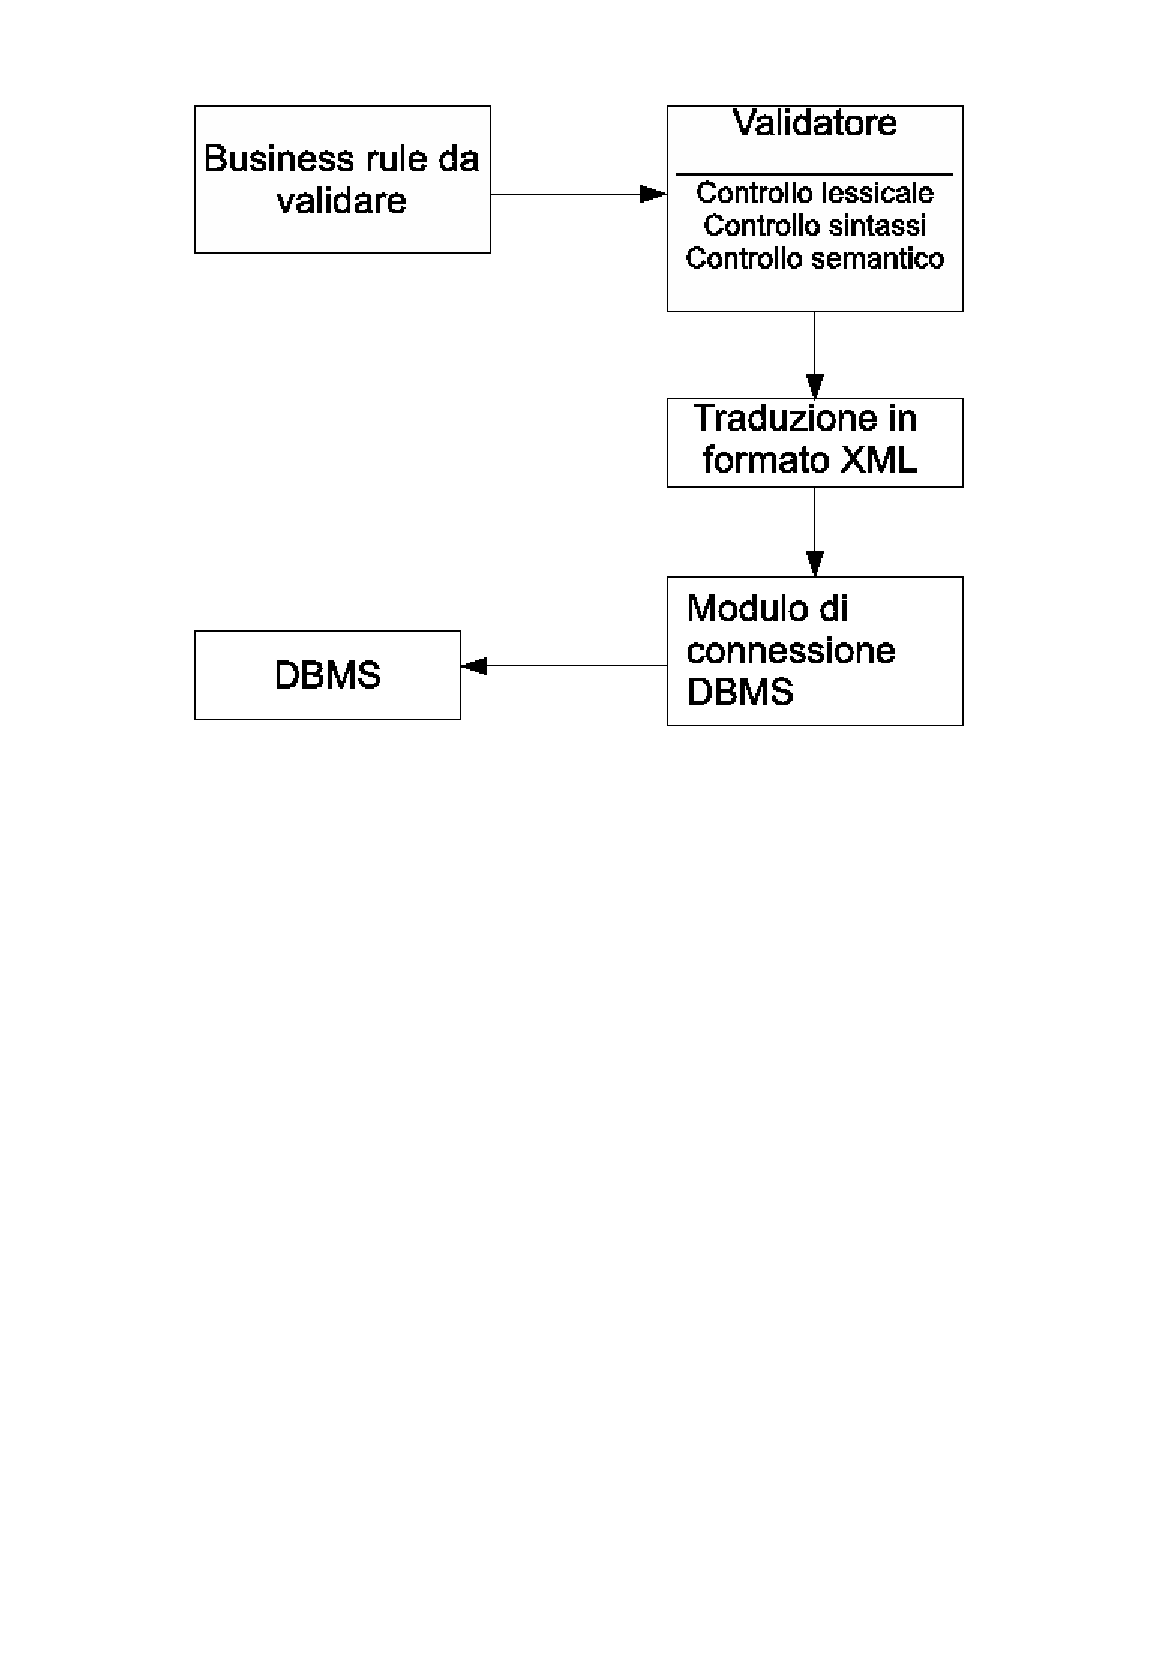
\includegraphics[width=1\textwidth]{st.eps}
\end{center}
Le istruzioni, tradotte in un formato interno dal validatore, descrivono cosa deve essere fatto e corrispondono alle istruzioni che l'interprete esterno deve effettuare sui business objects; tali istruzioni saranno quindi interpretate da quest'ultimo.
Le principali macro-componenti del sistema ``BR-jjsys'' sono:
\begin{itemize}
\item Validatore delle business-rules;
\item Modulo di connessione tra l'interprete e il DBMS (Database Managment System) esterno;
\end{itemize}

Questa suddivisione, per quanto minimale, consente di individuare le principali componenti che verranno ampliamente descritte nel successivo capitolo.

\chapter{Descrizione dei singoli componenti}
\subsection{Tipo, obiettivo e funzione del componente}

\begin{itemize}
\item Il validatore delle business-rules \`e un modulo software. Il suo obiettivo \`e verificare se la business-rules pu\`o essere inserita nel repository e, in caso affermativo tradurla in formato in XML comprensibile all'interprete esterno, altrimenti segnalare l'anomalia con  la rispettiva eccezione. Il nostro validatore ha un'architettura che comprende i seguenti sotto-componenti:
\begin{enumerate}
\item un analizzatore lessicale (lexer) che prende i token del nostro linguaggio e li traduce in una forma interna;
\item una tabella dei simboli che contiene le informazioni sui nomi delle entit\`a (variabili, nomi delle classi, nomi degli oggetti, etc.) utilizzate nel testo che si sta traducendo;
\item un analizzatore sintattico (parser) che controlla la sintassi del linguaggio che si sta traducendo: utilizza la grammatica del linguaggio da noi definita e costruisce l'albero sintattico;
\item un albero sintattico, ovvero una struttura interna che rappresenta il programma da compilare;
\item un analizzatore semantico che utilizza le informazioni dell'albero sintattico e la tabella dei simboli per verificare la correttezza semantica del testo in ingresso;
\item un generatore di codice che ``cammina'' sull'albero e genera il codice da inserire nel repository.
\end{enumerate}

\item Il modulo di connessione \`e un middleware, ovvero un programma che funge da intermediario tra l'interprete e il DBMS esterno. La sua funzione \`e quella di gestire la richiesta dell'interprete, inviandola al DBMS. Ricevute dal DBMS tutte le regole riguardanti un determinato business object, le invier\`a all'interprete esterno.
\item Interfaccia grafica (GUI) permetter\` all'utente di interagire con il validatore attraverso l'inserimento di nuove business rules e la cancellazione tramite la relativa chiamata al modulo di connessione.

\end{itemize}

\subsection{Relazioni d'uso di altre componenti}
Il modulo di connessione dialoga con la componente esterna DBMS attraverso il quale invia richieste di inserimento, cancellazione o recupero di informazioni. Ha relazioni inoltre con l'interprete esterno attraverso cui accetta richieste di business rules relative a un determinato business object. Successivamente il modulo di connessione chiama il DBMS richiedendo le opportune business rules che verranno restituite e inviate all'interprete. Il validatore dialoga con il DBMS esterno chiedendo di inserire le regole precedentemente validate. La GUI invece dialoga direttamente con il modulo di connessione durante la fase di cancellazione di una business rules e, direttamente con il validatore durante l'inserimento.

\subsection{Interfacce con e relazioni di uso da altre componenti}
Un interfaccia ``fornisce'' i servizi dal componente, ovvero i metodi che possono essere chiamati da un utente del programma. ``Specifica '' inoltre quali servizi devono essere forniti da altri componenti del sistema. Se questi non sono disponibili il componente non funzioner\`a senza per\`o compromettere l'indipendenza o la consegnabilit\`a di una componente, poich\`e non richiede che sia utilizzato uno specifico componente per fornire i servizi. Nel nostro caso:
\begin{itemize}
\item La componente GUI richieder\`a che l'interfaccia fornita comprenda i metodi per inserire, cancellare e cercare le business rules. Richieder\`a quindi un'interfaccia di gestione e un'interfaccia dati.
\item La componente validatore richieder\`a due interfaccie: di input e di output. La prima deve colloquiare tra l'utente e il validatore, la seconda dal validatore al modulo di connessione.
\item La componente modulo di connessione richieder\`a che l'interfaccia colloqui con l'interprete esterno.
\end{itemize}
\subsection{Attivit\`a svolte e dati trattati}


\chapter{Stime di fattibilit\`a e di bisogno di risorse}
Dopo aver analizzato il problema attraverso schemi progetturali sono state individuate le risorse necessarie  per la realizzazione del prodotto. Attraverso l'utilizzo di software open source siamo riusciti a contenere i costi e contemporaneamente a rendere disponibili tutte le risorse necessarie.
Le risorse necessarie ai nostri componenti per affrontare le varie problematiche di comunicazione, sviluppo del codice, gestione degli archivi, verifica dei documenti e del sistema sono state descritte nel documento Piano di Qualifica. Nella fase di specifica tecnica e successivamente di progettazione verrano utilizzati diagrammi UML delle classi e degli oggetti realizzati con Dia. Lo sviluppo avr\`a luogo singolarmente o in piccoli gruppi a seconda della natura della problematica da affrontare. Il documento/codice avr\`a in ogni modo un unico proprietario incaricato di renderlo pubblico tramite server SVN.

\chapter{Tracciamento della relazione componenti-requisiti}



\end{document}

    
